\begin{example}
Περιγράψτε το μετασχηματισμό που εκτελεί scaling ενός αντικειμένου ως προς ένα δοσμένο σταθερό σημείο $P(h,k)$ (Σχήμα 3.14). Το scaling να γίνει κατά $a$ μονάδες στον άξονα $x$ και κατά $b$ μονάδες στον άξονα $y$. Υπολογίστε το σχετικό πίνακα $S_{a,b,P}$ που θα εκτελεί το συγκεκριμένο μετασχηματισμό.
\end{example}
\begin{solution}

	
\begin{figure}[h!]
	\begin{center}
		\begin{minipage}[b]{0.45\textwidth} % Top-left image
		    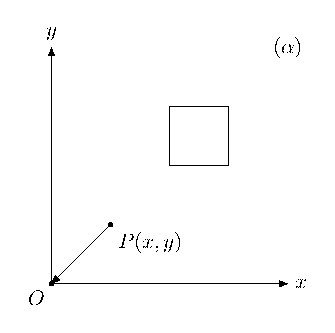
\includegraphics[width=\textwidth]{Chapter2/figure14a.pdf}
		\end{minipage}%
	\hfill
		\begin{minipage}[b]{0.45\textwidth} % Top-right image
		    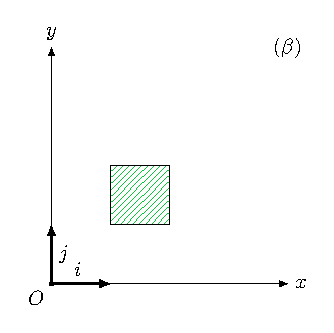
\includegraphics[width=\textwidth]{Chapter2/figure14b.pdf}
		\end{minipage}
	\end{center}
%\caption{Στρέβλωση ενός τετραγώνου για $a=2$ και $b=2$}
\end{figure}

\begin{figure}[h!]
	\begin{center}
		\begin{minipage}[b]{0.45\textwidth} % Top-left image
		    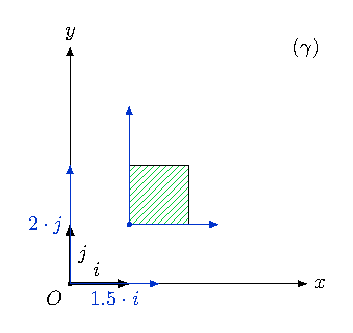
\includegraphics[width=\textwidth]{Chapter2/figure14c.pdf}
		\end{minipage}%
	\hfill
		\begin{minipage}[b]{0.45\textwidth} % Top-right image
		    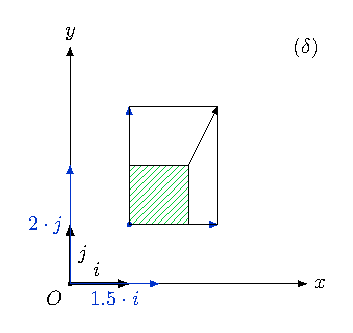
\includegraphics[width=\textwidth]{Chapter2/figure14d.pdf}
		\end{minipage}
	\end{center}
%\caption{Στρέβλωση ενός τετραγώνου για $a=2$ και $b=2$}
\end{figure}

\begin{figure}[h!]
	\begin{center}
		\begin{minipage}[b]{0.45\textwidth} % Top-left image
		    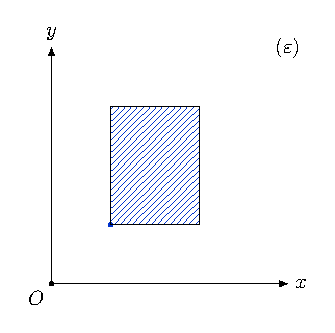
\includegraphics[width=\textwidth]{Chapter2/figure14e.pdf}
		\end{minipage}%
	\hfill
		\begin{minipage}[b]{0.45\textwidth} % Top-right image
		    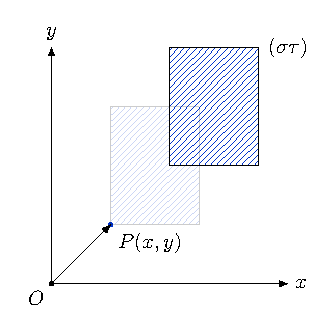
\includegraphics[width=\textwidth]{Chapter2/figure14f.pdf}
		\end{minipage}
	\end{center}
\end{figure}

Εφαρμόζουμε γεωμετρικούς μετασχηματισμούς. Θα προσπαθήσουμε να αναγάγουμε το ζητούμενο μετασχηματισμό σε σύνθεση βασικών μετασχηματισμών και ιδιαίτερα του βασικού scaling ως προς την αρχή των αξόνων. Εκτελούμε τα ακόλουθα βήματα:

Βήμα 1: Μεταφέρουμε το σταθερό σημείο $P$ στην αρχή των αξόνων. Η μεταφορά θα γίνει κατά διάνυσμα $-V$, όπου $V = h\hat{i} + k\hat{j}$, $\hat{i}$ και $\hat{j}$ τα μοναδιαία διανύσματα στους άξονες $x$ και $y$ αντίστοιχα (Σχήμα 3.14(b)).



\[
\text{Βασικός πίνακας μετασχηματισμού:} T_{-V}
\]

Βήμα 2: Εκτελούμε scaling ως προς την αρχή των αξόνων με $s_x = a$ και $s_y = b$ (Σχήμα 3.14(c)).

\[
\text{Βασικός πίνακας μετασχηματισμού: } S_{s_x, s_y}
\]

Βήμα 3: Επαναφέρουμε το σημείο $P$ στην αρχική του θέση. Η μεταφορά θα γίνει τώρα κατά διάνυσμα $V$ (Σχήμα 3.14(d)).

\[
\text{Βασικός πίνακας μετασχηματισμού: } T_V
\]

Ο ζητούμενος μετασχηματισμός θα προκύψει σαν σύνθεση των παραπάνω βασικών μετασχηματισμών:

\[
S_{a,b,P} = T_V \circ S_{s_x, s_y} \circ T_{-V}
\]

Αντικαθιστώντας τους βασικούς πίνακες μετασχηματισμών στην παραπάνω σχέση προκύπτει ότι:

\[
S_{a,b,P} =
\begin{bmatrix}
1 & 0 & h \\
0 & 1 & k \\
0 & 0 & 1
\end{bmatrix}
\cdot
\begin{bmatrix}
a & 0 & 0 \\
0 & b & 0 \\
0 & 0 & 1
\end{bmatrix}
\cdot
\begin{bmatrix}
1 & 0 & -h \\
0 & 1 & -k \\
0 & 0 & 1
\end{bmatrix}
=
\begin{bmatrix}
a & 0 & -ah + h \\
0 & b & -bk + k \\
0 & 0 & 1
\end{bmatrix}
\]

Οι συντεταγμένες των καινούργιων σημείων του αντικειμένου προκύπτουν από την επίδραση του $S_{a,b,P}$ πάνω στο αρχικό αντικείμενο.

Βασική παρατήρηση: Χρησιμοποιώντας το μετασχηματισμό $S_{a,b,P}$ μπορούμε να τροποποιήσουμε τις διαστάσεις ενός αντικειμένου διατηρώντας σταθερό ένα συγκεκριμένο σημείο του $P$.
\end{solution}